\chapter{Felhasználói dokumentáció} % User guide
\label{ch:user}

Ezen fejezet a felhasználó részletes tájékoztatására szolgál. Az alfejezetek az alkalmazás szükséges előfeltételeit, telepítési és használati információkat tartalmaznak. A program technikai részletekbe menő dokumentációját a \ref{ch:impl} . fejezet (Fejlesztői dokumentáció) tartalmazza.


\section{Röviden az agilis módszertanról és a  "scrum"-ról} % Briefly about the "scrum" 

\begin{description}
	\item[Mi az agilis módszertan?] A szoftverfejlesztési módszerek egy csoportja, ahol a követelmények és megoldások szoros együttműködésén keresztül fejlődnek az önszerveződő  és 		     	multifunkcionális csapatok. Ez elősegíti a korai szállítást, folytonos továbbfejlesztést és bátorít a változásokra adható gyors és rugalmas válaszokra. \footnote{Forrás: \url{https://www.agilealliance.org/agile101/}}
	\item[Mi a "scrum"?] Az agilis módszertanon belül sokféle irányzat van, ezek egyike a scrum. A scrum középpontjában a kis létszámú, önszerveződő agilis csapatok állnak. Itt,
 szemben a többi agilis ágazattal, nincsenek általánosan megszabott ,egész rendszert egybefogó szállítási és frissítési időpontok, hanem az aktuális fejlesztések \textbf{Sprintekbe} rendeződnek és ezek lejárta után történik az átadás. Ez közvetlenebb visszajelzést biztosít a szállító és a megrendelő között. A scrum szerkezeti felépítése a következő: van egy scrum master, aki egybe fogja a csapat működését, feladata a scrum "menedzselése" gyakorlatilag. Mellette a csapat tartalmaz természetesen fejlesztőket és tesztelőket. A scrum létszáma nincsen hivatalosan meghatározva, de ajánlatos 8-10 főnél nem nagyobbra nőnie, különben veszít hatékonyságából. A csapatok minden nap egy meghatározott időpontban tartanak "stand up"-okat, amelyeken minden tag beszámol feladatairól, haldásáról, így mindenki a csapaton belül képbe kerülhet a \textbf{Sprint} aktuális állásáról. Részletes összefoglalása olvasható: \cite{agilis}.
\end{description}

Pár fontosabb fogalom, amelyek a későbbiekben külön fejezetben részletezve lesznek:
\begin{itemize}
	\item Projekt \ref{projects}. fejezet
	\item Epic, User stories, Task, Issue \ref{stories}. fejezet
	\item Kanban \ref{kanbanboard}. fejezet
\end{itemize}

\newpage

\section{Rendszerkövetelmények} % System requirements

\textbf{Minimum követelmények}: A \textit{ScumHelper} egy webes alkalmazás. Ez azt jelenti, hogy a felhasználónak csak egy böngészőre van szüksége a számítógépén (például: Google Chrome, Mozilla Firefox, Safari, stb.) és természetesen internet elérésre ahhoz, hogy futtatni tudja a szoftvert. Utóbbi elengedhetetlen, ugyanis csak bejelentkezve lehetséges használni. Internet kapcsolat nélkül a számítógép csak a gyorsírótárában mentett oldalakat tudja megnyitni, de módosításokat nem tudunk végrehajtani a betöltött oldalon és új lapot sem tudunk megnyitni az alkalmazáson belül. Nincsen megkötés operációs rendszer tekintetében, tehát minden, napjainkban használatos rendszeren (Linux, Windows, Mac OS) egyaránt használható. 

\textbf{Ajánlott követelmények}: A jobb felhasználói élmény érdekében érdemes legalább 1280x720 felbontású kijelzőn használni és a korábban már felsorolt, jelenleg leggyorsabbnak és legbiztonságosabbnak számító böngészővel megnyitni : Chrome, Mozilla Firefox, Microsoft Edge, valamint érdemes széles sávú internet eléréssel rendelkezni.

\section{Telepítés}
\label{install}

A felhasználói oldalról nem igényel telepítést. Az eléréshez a szerver elérési URL-jére van szükség, illetve egy felhasználó igénylésére az aktuális rendszergazdától. Érdemes az új felhasználóba való belépés után megváltoztatni jelszavunkat biztonsági okokból.

Rendszergazdai oldalról ha még nem rendelkezik felhasználóval, akkor a fejlesztői dokumentációban (\ref{ch:impl}. fejezet) található információ a rendszergazda felhasználó létrehozásának lépéseiről.  Ha futtatni szeretné az alkalmazás szervert lokálisan, a saját számítógépen, vagy egy kihelyezett szervergépen, akkor azon telepíteni kell a következő programokat:  \textit{python} (3.5 vagy később verzió) \footnote{\url{https://www.python.org/downloads/}}, \textit{django és django-extension} python csomagok\footnote{\url{https://docs.djangoproject.com/en/3.0/intro/install/}}, valamint egy adatbázis kezelő szoftvert (PostgreSQL, Oracle, MySQL, MariaDB, SQLite).


\newpage

\section{Az alkalmazás felépítése}

\subsection{Bejelentkezés, felhasználók}

Az alkalmazásban az első képernyő, amely fogadja a felhasználót az a login oldal. A ScrumHelper-t csak sikeres bejelentkezés után lehetséges használni. Ha nem rendelkezik felhasználóval, akkor keresse meg a rendszergazdát, és igényeljen egyet. Az egyes felhasználói fiókok egy-egy jogosultsági csoporthoz kötöttek. 

A felhasználói csoportok és jogosultságaik:

\begin{table}[H]
	\centering
	\begin{tabular}{ | m{0.25\textwidth} | m{0.65\textwidth} | }
		\hline
		\textbf{Csoport} & \textbf{Jogosultságok} \\
		\hline \hline
		\emph{Fejlesztő} & projekt/epic/story/task/issue létrehozás/szerkesztés, komment létrehozás/törlés, saját munkaidő napló létrehozása/törlése, Dokumentum feltöltés (ha projekt tulajdonos, akkor törlés), jelszóváltás \\
		\hline
		\emph{Tesztelő} &   projekt/epic/story/task/issue létrehozás/szerkesztés, komment létrehozás/törlés, saját munkaidő napló létrehozása/törlése, Dokumentum feltöltés (ha projekt tulajdonos, akkor törlés), jelszóváltás \\
		\hline
		\emph{Scrum master} & projekt/epic/story/task/issue létrehozás/szerkesztés/törlés, komment létrehozás/törlés, saját munkaidő napló létrehozása/törlése/egész scrum könyvelés megjelenítése, Dokumentum feltöltés (ha projekt tulajdonos, akkor törlés), jelszóváltás \\
		\hline
		\emph{Projekt menedzser} & projekt/epic/story/task/issue létrehozás/szerkesztés/törlés, komment létrehozás/törlés, saját munkaidő napló létrehozása/törlése/egész scrum könyvelés megjelenítése, Dokumentum feltöltés (ha projekt tulajdonos, akkor törlés, jelszóváltás) \\
		\hline
		\emph{Rendszergazda} & minden jogosultsággal rendelkezik, létre is hozhat új csoportokat, kezelheti azok jogosultságait, illetve a felhasználókat is tudja szerkeszteni, vagy törölni \\
		\hline
	\end{tabular}
	\caption{Jogosultsági csoportok és jogosultságaik}
	\label{tab:example-1}
\end{table}

\subsection{Főoldal}

\begin{figure}[H]
	\centering
	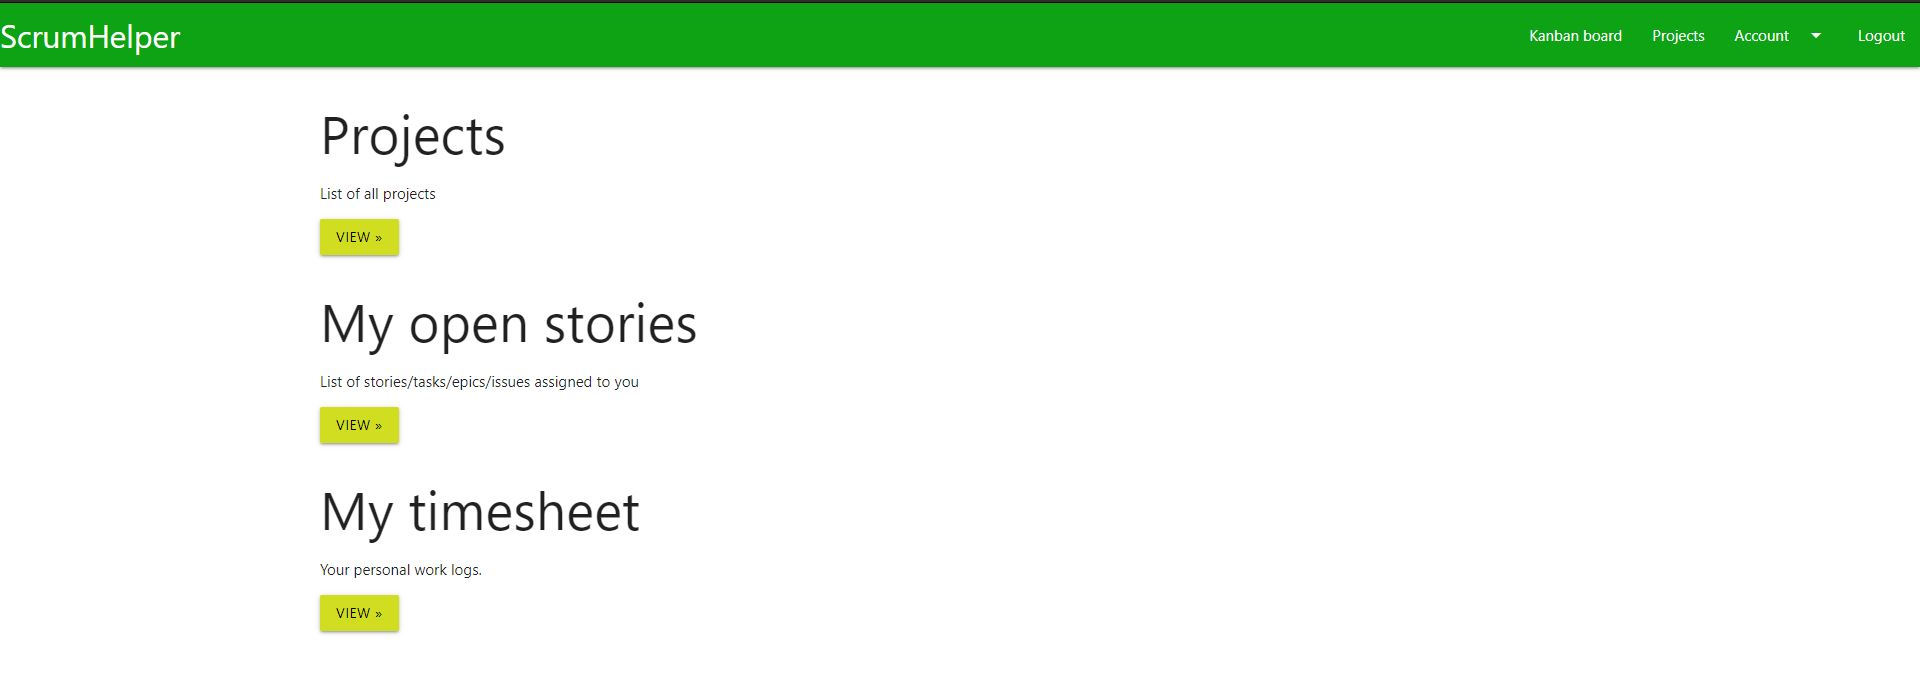
\includegraphics[width=1\textwidth,height=175px,frame]{index_page}
	\caption{Főoldal}
	\label{fig:example-1}
\end{figure}

A \ref{fig:example-1}. ábrán látható a főoldal kinézete. A navigációs sávban az alkalmazás neve, \textbf{Kanban board, Projects, Account} és \textbf{Logout} mezőket olvashatjuk. A \textbf{Kanban board} elnavigál a scrum Kanban táblájára, ahol az összes felvett feladatot láthatjuk egyben. A \textbf{Projects} menüponttal juthatunk el az adatbázisban szereplő projektek listájához. Az \textbf{Account} menüpont egy legördülő menü, amelyben a \ref{fig:example-2}. ábrán látható tartalom jelenik meg.

\begin{figure}[H]
	\centering
	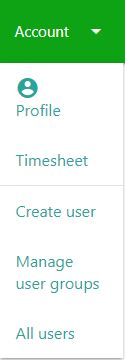
\includegraphics[scale=1]{account_dropdown}
	\caption{Account legördülő menü}
	\label{fig:example-2}
\end{figure}

Az elválasztó vonal alatti almenük: \textbf{Create user,  Manage user groups, All users} csak a rendszergazda jogosultságú felhasználók számára láthatóak. A \textbf{Logout} menüpont értelemszerűen kijelentkezteti a felhasználót és a bejelentkező oldalra ugrik.

A főoldal törzsében található 3 opció: \textbf{Projects} - a \textbf{Projects} menüponttal megegyezően a projektek listájára navigál, \textbf{My open stories} - a bejelentkezett felhasználóhoz rendelt story-k/task-ok/issue-k tekinthetőek meg és a profil adatok, \textbf{My timesheet} - a felhasználó munkaidő könyvelési oldalára kalauzol.

\subsection{Projektek}
\label{projects}

A projektek listájához a \textbf{Projects} menüpontból, illetve a főoldalról tudunk eljutni. Az oldalon egyszerre 5 projekt jelenik meg, a többit a \ref{fig:example-3}.ábra alján látható oldal léptetéssel érhetjük el. A projektek létrehozási dátum szerint a legújabbtól haladva a legrégebbi felé jelennek meg. A projekt oldalak esetében a navigációs sávban is megjelenik egy "Create project" feliratú gomb, mellyel egyből a létrehozás oldalra juthatunk.

\begin{figure}[H]
	\centering
	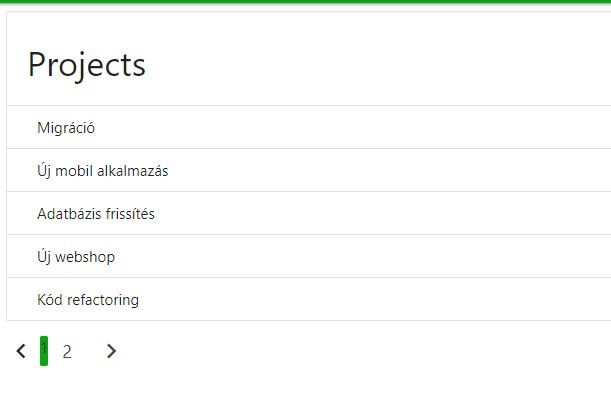
\includegraphics[scale=0.75]{project_list}
	\caption{Projektek listája}
	\label{fig:example-3}
\end{figure}

Az egyes projektekre kattintva eljutunk a projektek saját oldalára. Itt megtalálhatjuk az alapvető információkat a projektről, a projekthez feltöltött dokumentumokat, valamint a projekthez tartozó összes feladat (epic,story,task,issue) felsorolását egy görgethető listában. A jobb alsó sarokban található egy menü, mely az egyes feladat fajták saját oldalain is megtalálhatóak, természetesen részben eltérő menüpontokkal. A projektek esetében ez tartalmazza a szerkesztés, epic, story, task, issue létrehozásait, illetve a megfelelő jogosultsággal rendelkezőknek a törlés opciót. (\ref{fig:example-4}. ábra).

\begin{figure}[H]
	\centering
	
\includegraphics[scale=0.75]{edit_menu}
	\caption{almenü, mely különböző opciókat tartalmaz projekt, vagy feladat típustól függően}
	\label{fig:example-4}
\end{figure}

\subsection{Epic, Story, Task, Issue}
\label{stories}

\begin{figure}[H]
	\centering
	\subfigure[Epic]{
		
\includegraphics[scale=1]{epic}}
	\hspace{35pt}
	\subfigure[Story]{
		
\includegraphics[scale=1]{story}}
	\hspace{35pt}
	\subfigure[Task]{
		
\includegraphics[scale=1]{task}}
	\hspace{35pt}
	\subfigure[Issue]{
		
\includegraphics[scale=1]{issue}}
	\caption{Az egyes feladat típusok ikonjai}
	\label{fig:example-5}
\end{figure}


\begin{description}
	\item[Epic:] Egy projekten belül levő feladatok gyűjteménye. Mivel projektek több sprinten át élhetnek, ezért rövidebb időszakokban az összefüggő story-k és task-ok összefogására érdemes ezt használni. Létrehozni az adott projekt oldalán, a korábban említett almenüből lehet (\ref{fig:example-4}. ábra). 
	\item[Story:] Felhasználói feladat. Ha valamilyen jól körülhatárolt fejlesztés van a projekten belül, akkor érdemes ezt használni annak leírására. Létrehozatalkor még nem kötelező hozzárendelni felhasználót, azt lehet később is a story szerkesztésével. Létrehozni a projekt oldalán levő almenüből (\ref{fig:example-4}. ábra) lehetséges, vagy egy adott epic saját oldalán levő almenüből (story ikonjára kattintva), illetve a navigációs sávban megjelenő \textbf{Create story} gombra kattintva. Ez olyankor elérhető, amikor egy meglévő story oldalán vagyunk éppen.
	\item[Task:] Szintén felhasználói feladat. A task-ot a story-val ellentétben kisebb feladatok leírására érdemes használni. Például, ha valaki dokumentációt ír, vagy meetingekre jár, vagy csak valami apró fejlesztésről van szó, akkor érdemes azt "taskosítani". Létrehozni a projektek, illetve epic-ek és story-k oldalán lehetséges az almenüből (\ref{fig:example-4}. ábra) a task ikonjára kattintva.
	\item[Issue:] Az issue kicsit eltér a story-tól és a task-tól. Az issue valamilyen jellegű hiba leírására használható. Például, ha egy elkészült fejlesztésben a tesztelő hibát talál, vagy ha már a leszállított build-ben derül ki valamiféle "bug". Létrehozni a projekt almenüjében lehetséges (\ref{fig:example-4}. ábra).
\end{description}

A story, task és issue hármas státusszal is rendelkezik. Az aktuális státuszt minden olyan oldalon láthatjuk, ahol valamilyen felsorolásban szerepel a 3 közül bármely feladat típus. A státuszt az adott feladat saját oldalán lehet a jobb felső sarokban látható gombbal állítani, melyen mindig az a státusz olvasható, amely az éppen aktuálisat követi.

\begin{figure}[H]
	\centering
	
\includegraphics[scale=1]{storyExample}
	\caption{Példa egy story-ra egy felsorolásban: látható a neve, a projekt kódja, ikonja és aktuális státusza}
	\label{fig:example-6}
\end{figure}

\subsection{Egy példa fejlesztési ciklus}
\label{example_workflow}

Az egyes fogalmak gyorsabb és könnyebb megértése érdekében egy példa fejlesztési folyamat a szemléltetés céljából:

\begin{enumerate}
	\item A scrum masterhez megérkezik a fejlesztési igény (projekt) a megrendelőtől.
	\item Felvesz egy projektet a \textit{ScrumHelper}-ben. Feltölti hozzá az igényhez kapott dokumentumokat, amelyek segítik majd a tervezők munkáját. \textbf{Projects} menüpont a navigációs sávban (vagy a Főoldalon) -> \textbf{Create project} sárga gomb a navigációs sávban -> A formula helyes kitöltése és \textbf{Submit} gomb -> Az új projekt oldalán a \textbf{File} gombra kattitnva kiválasztja a fájlt, amit fel akar tölteni, majd rányom a gémkapocs ikonnal rendelkező gombra.
	\item Ezt követően kiosztja az igény megtervezését egy tervezőnek (architect). Ehhez task-ot készít, ahol összeírja a teendőket röviden. Az új projekt oldalán a jobb alsó menüből, a \textbf{Task} ikonjára kattint (kék alapon fehér könyvjelző) -> Kitölti a \textbf{Task} kreáló formulát, az \textit{assignee} mezőben a tervező felhasználóját adja meg -> rányom a \textbf{Submit} gombra
	\item A tervező megírja az igény specifikációját arról, hogyan lehetne ezt az adott rendszerben implementálni (High Level Solution Design).
	\item Utóbbit feltölti a projekt többi dokumentumai közé, majd elkezdi lebontani feladatcsoportokra (epic) és feladatokra (story). Hasonlóan a 2. lépésben leírtakhoz, a projekt oldalán feltölti a fájlt -> Az almenüben az \textbf{Epic} ikonjára kattint (lila alapon fehér négyzet), vagy a \textbf{Story} ikonjára kattint (zöld alapon fehér diagramm) -> kitölti a formulákat és a \textbf{Submit} gombra nyom -> létrejönnek az új feladatok a projekthez.
	\item A fejlesztő ezután válogathat a story-k között, melyiket szeretné megcsinálni. Amelyiket kiválasztja azt magához rendeli a story szerkesztői oldalán és IN PROGRESS-be rakja a státuszt. \textbf{Projects} menüpontból, avagy a főoldalról elnavigál a projekt oldalára, vagy a \textbf{Kanban board} menüponttal megtekinti a kanban táblán az aktuálsi feladatokat -> kiválaszt egyet a listákból és az adott feladat saját oldalán az almenüben a szerkeztés gombra kattint (sárga alapon fehér toll) -> az \textit{assignee} mezőben kiválasztja a saját felhasználóját -> \textbf{Submit} gomb. -> a feladat (Story) saját oldalán a státusz gombbal IN PROGRESS státuszba helyezi azt.
	\item Amint végzett a fejlesztéssel, TESTING státuszba állítja. Egy tesztelő megkeresi (például a Kanban boardon) és magához rendeli. A fejlesztő a feladat oldalán rányom a \textbf{TESTING} feliratú gombra -> a tesztelő a \textbf{Kanban board} menüpontbeli kanban táblán megkeresi a TESTING státuszú feladatok között -> rákattintva eljut annak saját oldalára -> a jobb alsó menüben rányom a szerkesztés ikonjára (sárga alapon fehér toll) és az \textit{assignee} mezőt a saját felhasználójára állítja.
	\item Ha tesztelés közben hibát talál, akkor felvesz a projekthez egy issue-t amit az eredeti fejlesztőhöz (vagy aki javítani tudja) rendeli. Érintett projekt saját oldala -> almenüben issue ikonja (piros alapon fehér felkiáltójel) -> Formula megfelelő kitöltése (helyes hibatípus kiválasztása, fejlesztőhöz rendelés) és \textbf{Submit} gomb.
	\item Amikor már nincsen probléma a story-val, akkor DONE státuszba rakja. \textbf{Story} saját oldala -> \textbf{DONE} feliratú gomb
	\item Egy feladat életciklusának utolsó állomása a CLOSED, amelyre a sprint végén ajánlatos állítani. Ha valami okból újra foglalkozni kell vele, akkor lehetőség van a REOPEN opcióval újra nyitottá tenni. \textbf{Story} saját oldala -> \textbf{CLOSE} feliratú gomb
\end{enumerate}

\subsection{Kanban tábla}
\label{kanbanboard}

A \textit{kanban} szintén egy egységesen használt fogalom (avagy eszköz) a scrum módszertanban. A kanban board - azaz "tábla" - arra szolgál, hogy egybe gyűjtse a scrum összes felvett feladat típusát. A \textit{ScrumHelper}-ben ez a funkció a navigációs sávban a \textbf{Kanban board} menüpontra kattintva érhető el. Itt négy státusz alapján négy oszlopra osztva láthatóak az aktuális (DONE státuszban csak a 30 napon belül módosultak maradnak megjelenítve) feladatok: OPEN (nyitott), IN PROGRESS (folyamatban), TESTING (tesztelés alatt), DONE (kész).

\begin{figure}[H]
	\centering
	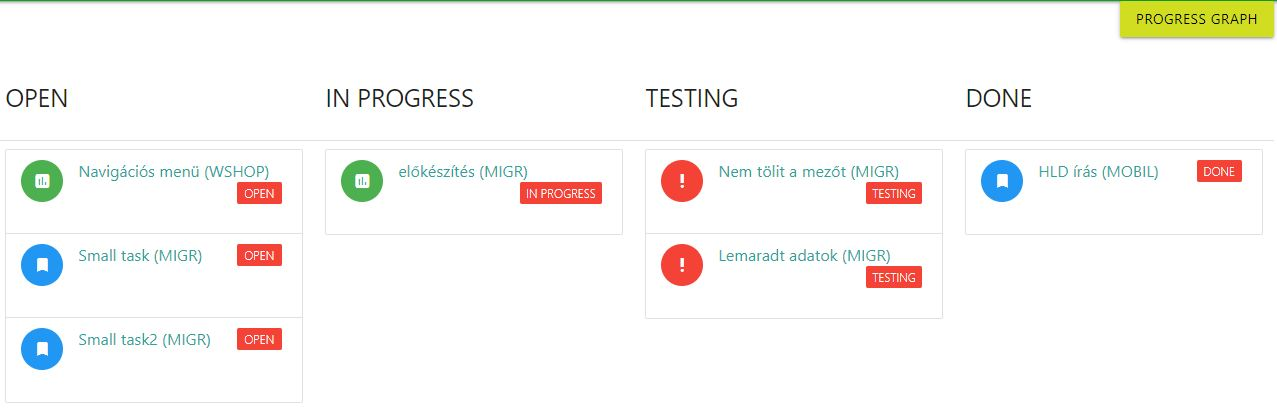
\includegraphics[width=1\textwidth,height=175px,frame]{kanban}
	\caption{Kanban tábla}
	\label{fig:kanban}
\end{figure}

A jobb felső sarokban látható gomb ( \ref{fig:kanban}. ábra "Progress graph") megnyomásával egy körgrafikon segít az aktuális feladatok állásának nyomon követésében. Az alábbi ábrán egy példa:

\begin{figure}[H]
	\centering
	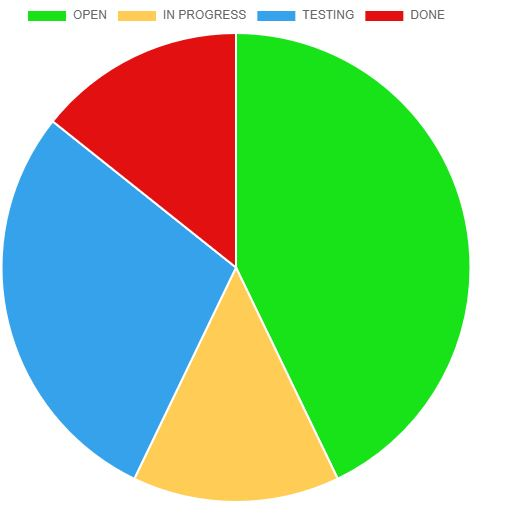
\includegraphics[scale=0.75]{chart}
	\caption{Körgrafikon az aktuális feladatok jelen státuszáról}
	\label{fig:kanbanchart}
\end{figure}

\subsection{Munkanapló}
\label{worklog}

Az alkalmazás lehetőséget biztosít az egyes feladatokkal eltöltött munkaidő számontartására is. Ehhez el kell navigálniuk az adott feladat (story, task, issue) oldalára és a már korábban többször is említett (\ref{fig:example-4}. ábra), jobb alsó sarokban található almenüben kiválasztani a munkaidő könyvelése opciót ("Add worklog", ikon: kék körben fehér aktatáska). Ez eljuttatja a felhasználót a munkanapló bejegyzés létrehozó oldalára. Itt a dátum mezőt megfelelő formátumban kitöltve, avagy a naptár ikont használva meg kell adni a munkanapot. Alatta pedig megadni a feladattal töltött munkaórák számát, amely 1 és 8 közé kell essen. Ettől eltérő bemenetre figyelmeztet az alkalmazás, hogy rossz adatot adott meg. A navigációs sáv \textbf{Account} menüpont legördülő menüjében (\ref{fig:example-2}. ábra) a \textbf{Timesheet} opcióra kattintva, avagy a főoldalról a \textbf{Timesheet} pontra kattintva tekinthető meg a saját profilunkhoz rögzített összes munkanapló bejegyzés napi és havi bontásban (\ref{fig:personaltimesheet}. ábra).

\begin{figure}[H]
	\centering
	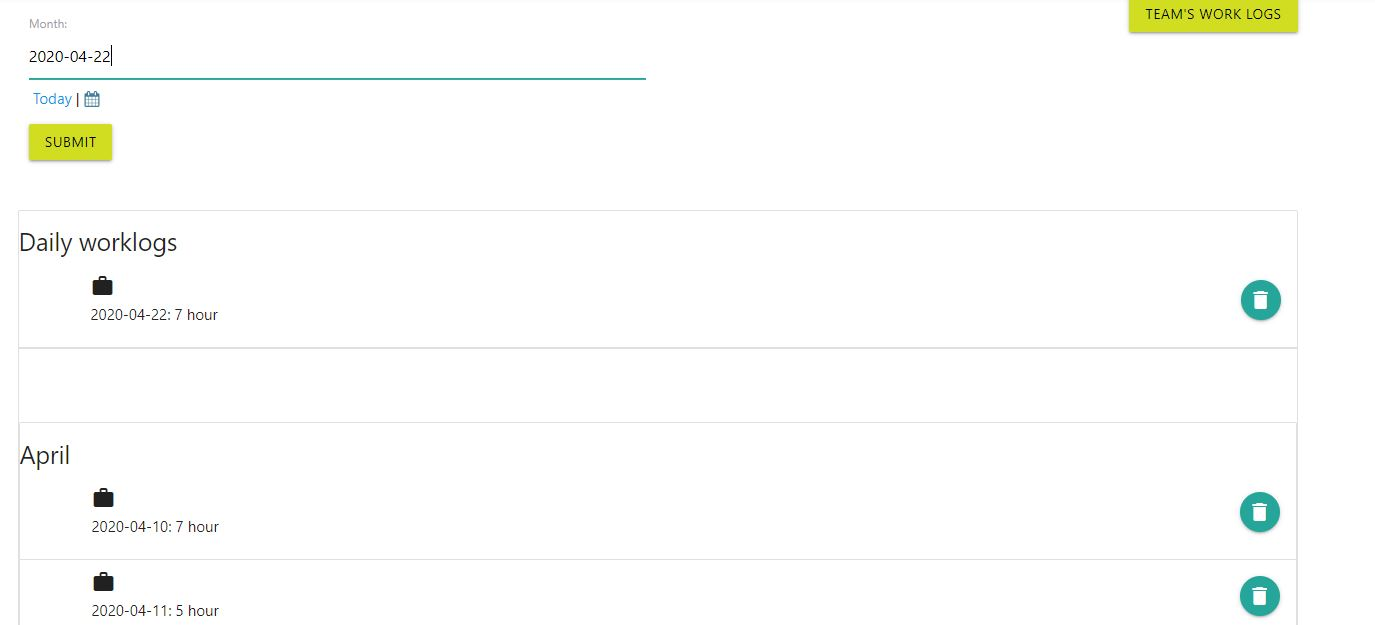
\includegraphics[width=1\textwidth,height=175px,frame]{owntimesheet}
	\caption{Személyes munkanapló}
	\label{fig:personaltimesheet}
\end{figure}

Kiválasztható a dátum napi pontossággal, akár kézzel beírva a megfelelő formátumban, akár a naptár ikonra kattintva a felugró naptárból. A jobb felső sarokban látható egy "TEAM'S WORK LOGS" feliratú gomb. Erre kattintva megtekinthető az egész scrum havi munkaidő könyvelése (\ref{fig:teamtimesheet}. ábra). Az egyéni naplóhoz hasonlóan, egy megadott dátum alapján az adott hónapra megjeleníti az egyes felhasználók által lekönyvelt összóraszámát. A jogosultságoknál említettek alapján, csak a scrum masterek, a projektmenedzserek és a rendszergazdák látják ténylegesen minden csapattag óraszámát. A többi csoport csak a sajátját látja összegezve. Törölni bejegyzést minden felhasználó csak maga tud, nem lehet másét eltávolítani. Ezt a személyes munkanapló oldalon lehet megtenni az egyes bejegyzés melletti kuka ikonra kattintva.

\begin{figure}[H]
	\centering
	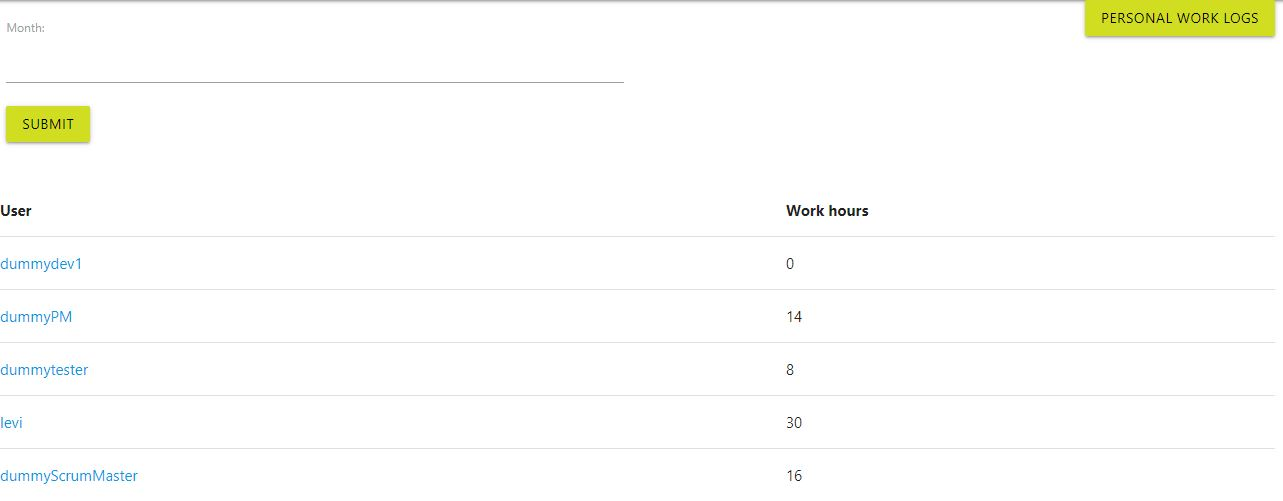
\includegraphics[width=1\textwidth,height=175px,frame]{teamtimesheet}
	\caption{Scrum felhasználóinak összmunkaórája az adott hónapban (amit a scrum master lát)}
	\label{fig:teamtimesheet}
\end{figure}

\newpage
